\documentclass{standalone}

\usepackage{placeins}

\begin{document}
	Firstly, throughout development Git has been used for version control; the repository is hosted on GitHub\parencite{TronGitRepo}. A todo-list full of various development tasks exists within the root directory of the repository. This helped to maintain an efficient workflow and to document thoughts for later development sessions. Efforts were also made to document and lint all produced source-code.

	The produced implementation consist of many aspects, most of which can be categorised into one of three groups: game mechanics, network communications and artificial intelligence. Thus, where possible, we shall try to discuss each one of these categories separately. However, before that we shall first provide an overview of the application and describe the relation between some of its core components.

	As the game is to be played in a web-browser, we will be making use of the three fundamental web languages, those being HTML, CSS, and JavaScript. These three languages, and the standards which govern them, allow us to confidently write portable code which will run identically within the majority of web-browsers. Sadly, this isn't always the case as many browsers do not support the most up-to-date standard; assuming it follows it in the first place...

	Now, the majority of our game, for the client-side at least, is programmed in JavaScript; allowing it to run in web-browsers. However, due to the compatibility issues mentioned above, we have wrote our game according to the ECMAScript2015 standard \parencite{ECMAScript2015} and transpile it to a more commonly supported syntax using Babel\parencite{Babel}.

	Transpiling to JavaScript has become somewhat the norm in the realm of modern front-end web-development. In recent years, many new programming languages have in fact emerged under the sole purpose of being transpiled into JavaScript. The reason we chose not to use one of these new languages is because it masks away a lot of the underlying code which the browser is expected to run; creating another layer for things to potentially go wrong.

	As the game was to be built for a web-browser, we already have access to a wide range of graphical components, as per the HTML specification. These are useful for components such as buttons and lists. However, it is quite cumbersome to maintain a proper reflection of our game's state (which resides within the JavaScript environment) onto our DOM. This is quite a frequent issue with web-applications and is the basis for many very popular frameworks. With this in mind, along with desire to learn a new framework and the curiosity to find out as to how helpful it would be with this project; React\parencite{React} and Redux\parencite{Redux} have been used to help handle the view layer.

	Given that we already have to use Javascript for our front-end game code, it makes sense to not bring in another language for our back-end. This has a myriad of benefits including not having to deal with the additional quirks of a separate programming language and eliminating the hassle of maintaining two separate implementations of code that is identical in purpose. Hence for the back-end, on the server, we use Node.js\parencite{NodeJs}.

	Somewhere early on during development, having already settled on the aforementioned technologies, it began more and more difficult to maintain an efficient work-flow whilst developing. That inspired the decision to transition the project to use the React Universally \parencite{ReactUniversally} starter-kit; a boilerplate project with a bare-bones project base structure and various scripts to help automate the tedious build/watch process.

	React Universally also sets up Server-side rendering with React. This is helpful as it enables the server to perform an initial render of our application's components, then serve the result to the client. This makes the web-page appear to load faster, as the client is no longer required to perform this initial render themselves; they just mount the components then rehydrate the state.

	The source code is split into three main directories: \emph{shared}, \emph{client}, and \emph{server}. The \emph{shared} directory contains the bulk of our application, including source which is rendered server-side to be served to a client. Whilst the \emph{client} directory is for browser specific source that will not be used server-side or for the purpose of server-side rendering. Similarly, \emph{server} is for source which is executed on our node server.

	\section{Game Mechanics}
		The source-code for Tron's game mechanics exist primarily within the \emph{game} sub-directory inside \emph{shared}. There have been attempts to keep it as decoupled as possible from the various libraries we've brought in. This was done to help reduce the risk of delay caused by a library that isn't explicitly required for the main goal of the application.

		The entire game state is stored within a single mutable JavaScript object. There exist numerous operations which can be applied to the state, each in the form of a function that take the state and additional parameters, if applicable. For the case when mutability is not desired, there exists a \emph{copyState} operation which explicitly copies the entire state and rebuilds the cache.

		Below is a breakdown of the structure for our game state object:
		\begin{description}
        \item[tick]: the number of times this state has ticked; inclusive of the current tick update.
        \item[progress]: the amount of time which has passed since the last tick update.
        \item[started]: a boolean indicating if a round of Tron is in progress.
        \item[finished]: a boolean indicating if the current round has finished. \emph{undefined} if started is \emph{false}.
        \item[arenaSize]: the number of cells within our game arena.
        \item[playerSize]: the number of cells a player occupies within our game arena.
        \item[speed]: the number of cells each player travels over the course of a millisecond.
        \item[players]: an array containing an object for each player part of the current game. The following describes the structure of a single player object:
        \begin{description}
        	\item[id]: a unique string used to identify the player.
        	\item[name]: an arbitrary string for other players to recognise this player.
        	\item[alive]: a boolean indicating if the player is alive, or otherwise dead.
        	\item[direction]: the direction (north, south, east, or west) in which the player is travelling.
        	\item[position]: a \emph{point} (an array, in the form of [\emph{x, y}]), representing the player's current position in the grid.
        	\item[trail]: an array of \emph{points} at which the player has changed direction. Used to construct a path of the area in which the player has travelled. However, the array has two special cases: the first element is the player's spawn point, and the last element is the point for the player's previous position.
      	\end{description}
        \item[cache]: a nested object containing various cache structures required by our state. The following describes the structure of the cache object:
        \begin{description}
        	\item[collisionStruct]: a data-structure in which we can check for player/trail collisions within our arena. See for more detail \fullref{collisionDetection}.
      	\end{description}
    \end{description}

		\subsection{Game Loop}
			The game loop is of a critical importance, it is charged with updating our game state and redrawing the graphics repeatedly at some fixed interval; known as a \emph{tick}. In principle, this entails calling some function continuously at some fixed rate.

			Both the client and server each implement their game loops slightly differently. The server needs to run fast enough to process user input and calculate updates with minimal perceptible latency. Whilst the client just runs with the purpose of redrawing the scene fast enough to create the illusion of smooth game-play. By default, both the client's and server's game loop runs at a tick-rate of once every 15 milliseconds - approximately 66 times a second. \footnote{This is considered the standard for video-games; faster rates, in most cases, have near indistinguishable benefit.}

		\subsection{Collision Detection} \label{collisionDetection}
			Many existing Tron implementations internally use a grid-based arena, that is a play occupies an entire whole cell of the arena. This enables collision look-ups to be performed in constant time, by simply indexing an array. However, our implementation allows players to move with an incredibly high-degree of precision\parencite{JsNumbers}. Unfortunately, this does complicate collision lookups.

			Instead of checking for collisions against every object in the arena, we have utilised the uniform grid spatial data-structure. This allows us to divide the arena into a grid of arrays, where each array holds references to the objects that reside within its bounded space. Thus, when checking for a collision, we only need to check against objects that are held within the array(s) that our target object intersects with; reducing the search space quite substantially.

			To populate our collision data-structure, we generate a series of rectangles representing each individual line-segment that forms the player's trail - from their current position, to the position they were spawned at. This is the stage at which we take into account the players' size.

			\begin{figure}[!htbp]
				\centering
				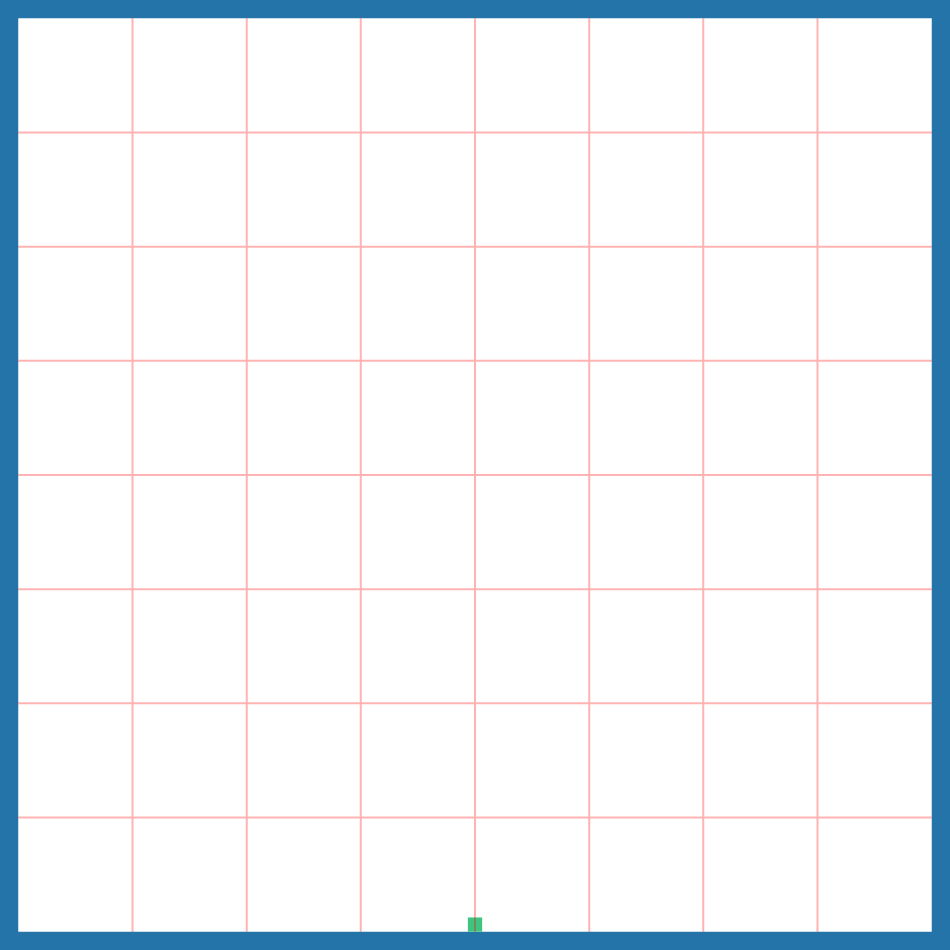
\includegraphics[width=.8\textwidth]{resources/images/uniformgrid.png}
				\caption{Visualisation of uniform-grid data-structure, drawn by our game's draw debug mode.}
			\end{figure}
			\FloatBarrier

			Once the search space has been reduced, we now need to check to see if any of the obtained objects collide with our target object. Conceptually, this is just checking if there exists an overlap between two rectangles; a very simple calculation. However, as we want players to stop at the precise moment at which they crashed, we must calculate the intersection point and then offset it appropriately using the size of the two players.

			This boils down to two distinct cases: \footnote{Please note that, in our collision case diagrams, the black dot within a player represents their position point. \label{blackDotDiagram}}
			\begin{enumerate}
    		\item
    			\textbf{Case}: player collides with another player - who is not heading in an opposing direction.\\
					\textbf{Solution}: reposition the crashed player by appropriately calculating an offset distance from the player they hit - based upon both their sizes. Using the crashed player's travelling direction for the offset's sign. \\
					\begin{minipage}{\linewidth}
						\centering
						\captionsetup{width=.8\linewidth}
	          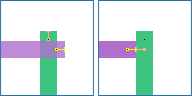
\includegraphics[width=.8\linewidth]{resources/images/collision/side.png}%
	          \captionof{figure}{Example of a sideways collision. On the left, two players are depicted in their unfixed positions. Whilst on the right, they're now shown in their relative position.}
	    		\end{minipage}
				\item 
					\textbf{Case}: head-on collision between two players.\\
					\textbf{Solution}: move each player backwards by half the sum of their \emph{overlap} and \emph{overshoot}.\\
					\begin{minipage}{\linewidth}
						\centering
						\captionsetup{width=.8\linewidth}
	          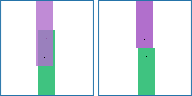
\includegraphics[width=.8\linewidth]{resources/images/collision/headon.png}%
	          \captionof{figure}{Example of a head-on collision. On the left, two players are depicted in their unfixed positions. Whilst on the right, they're now shown in their relative position.}
	    		\end{minipage}
			\end{enumerate}

	\section{Network Communication}
		For a game to be multiplayer, all players need to share the same consistent experience across a network, i.e. they need to all be playing on the same game state. So this raises the question on how to synchronise the game state between all connected players. There are two main methods to achieve a synchronised game state and, to some degree, we will be using ideas from both.

		The first method is known as \emph{peer-to-peer lockstep}. It centres around the idea of the game being modelled as turn-based and, before each turn, all non-deterministic events (such as user-input) are broadcasted to all players. Once all players have sent their input for this turn, each player then individually updates their game state; which will of course all end up being identical. The primary flaw in this technique is that all players are forced to play at the latency of the player with the weakest connection. This would be extremely frustrating for Tron, as each time you try to move you have to wait for the player with the weakest connection.

		The second method is known as \emph{client/server}. It entails having a single authoritative game-state kept on a server, that is then communicated between all players. When a player wants to perform an action, they must communicate said action to the server. The server will then apply the action and communicate the updated state to all connected players. However, this solution makes no compromises for latency. For example, the server's state is forever being updated and it will often receive actions from connected players that were made under the assumption the game is still at some previous state.

		Our developed solution entails the use of several techniques. At its core, it is a client-server model. But we make use of two mechanisms known as \emph{lag compensation}\parencite{LagCompensation} and \emph{client-side prediction}\parencite{LagPrediction} which help to reduce the negative effects of latency.

		Simply put, lag compensation enables the server to `rewind` time when applying the input of a user; compensating for any latency that may have occurred. Whilst lag prediction allows clients to mimic the server, including the immediate processing of their input. See \parencite{LatencyCompensating} for a more thorough description.

		Communicating the entire game state after each tick is an incredibly infeasible task; each player would be required to communicate with the server at a rate faster than the game's tick-rate.

		Our solution to this problem is quite a simple one. When the client receives a message containing the updated state, they immediately reply to the server with an acknowledgement. The server will interpret this acknowledgement as a request to prepare the next state transmission.

		To further reduce the latency of communication, we can also reduce the payload size of each state transmission. This is made possible by identifying that over the course of several ticks, the game state remains largely unchanged. Knowing this, we are able to keep in memory the last state communicated to each player and when we need to transmit, just calculate a snapshot of the differences \footnote{We calculate and apply the differences using \emph{fast-json-patch}\parencite{FastJsonPatch}.} between the current state and the last one which was sent. We also don't bother sending the cache, and instead simply regenerate it on the client - which isn't too expensive of an operation, and doesn't hinder our server's authoritative game state.

	\section{Artificial Intelligence}
		In order for our computer opponent to play the game, they need to be controlled by some artificial intelligence; some program which has an understanding of the game and can make sensible moves, as if it were a human player. This is quite a complicated, especially given that our game is played in real-time.

		Our solution to this problem centres around the idea of the modelling the game to be both played on a grid and turn-based, then running simulations which play out the possible scenarios in which the game could develop. However, as we require our AI to make decisions within a very short amount of time, we are unable to check the entire search-space and instead must make use of a variety of techniques to help optimise the process.

		Probably the most radical technique is to only run each simulation up until some fixed depth, at which point we then evaluate the current game state using an heuristic evaluation function. The effectiveness of this technique is heavily reliant on both the chosen fixed depth as well as the evaluation function.

		The heuristic evaluation function we've designed uses an optimised version of the flood-fill algorithm, featured in the very high-performing implementation that was the winner of a Google AI competition - introduced in \fullref{sec:background-google-ai}. The core idea is to count player \emph{ownership} of grid-cells, in our model of the arena, based upon a heuristic distance measurement.

		First, all players have their heuristic score initialised to 0. Then we calculate the minimum Manhattan distance between the AI player and all other alive players. We then apply flood-fill to calculate the distance from the current player to each empty grid-cell. Flood-fill is optimised by halting its process once the distance surpasses the previously calculated minimum distance. We are now left with a heuristic distance measurement.

		For each grid-cell, we then apply the following process to score based upon cell ownership: for each player, increment 1 to their score for every other player that has a distance that is greater-than, or equal to, the current cell. If the other player does not have a recorded distance to the current cell, instead increment by 2.

		Thus, a greater score indicates a stronger position; although not relative to other players.

		Even with the reduction in search-space and optimised evaluation function, time is still limited. So, we use Monte Carlo tree search \parencite{MonteCarloTreeSearch} with UCB1 to only explore promising branches of the game tree. 
		\begin{figure}[!htbp]
			\centering
			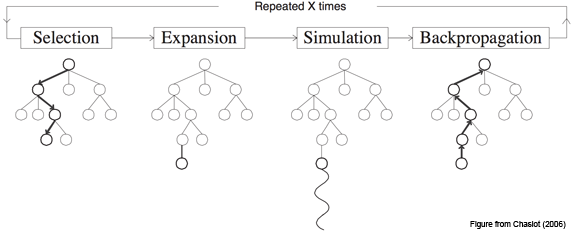
\includegraphics[width=.8\textwidth]{resources/images/mcts.png}
			\caption{Diagram depicting the Monte Carlo tree search algorithm, from \parencite{MonteCarloTreeSearchDiagram}.}
		\end{figure}
\end{document}